\chapter{Analysis of features and security requirements}
\label{requirements}

\subsection{TO ADD}
From EOF + Latency "`low"', eventual consistency

\subsubsection{Steganographic}
Not for hiding, but to support longer überleben?
http is pretty well suited for this.
mixing with smtp, imap, pop3, tcp. etc.


% -----------------------------------------------------------------------------
From the previous analysis of chat systems and related communication protocols,
several drawbacks can be seen. Most systems suffer a single point of failure,
which is due to the central architecture. Further the message content is often
neither protected nor verified.

The following security features are derived from the weaknesses of the previously
analysed systems as well from the thesis objectives.
% -----------------------------------------------------------------------------
\section{Anonymity}
There are four different types of anonymity:
\begin{itemize}
\item Pseudonymity
\item Sender anonymity
\item Receiver anonymity
\item Sender-receiver anonymity
\end{itemize}
Pseudonymity describes anonymity by using a different identity, for instance
\textit{telmich} instead of Nico Schottelius.
Sender anonymity is present, if nobody can observe who the sender is.
\begin{figure}
    \centering
    \caption[Sender Anonymity]{Sender Anonymity\\Image source: \protect\url{http://www.cs.virginia.edu/crab/anonymity.ppt}}
    \label{senderanon}
    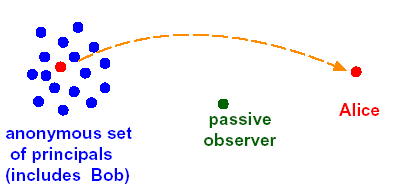
\includegraphics[scale=0.8]{sender-anon.png}
\end{figure}
Receiver anonymity is given, if an observer cannot identify  the receiver of
a message. 
\begin{figure}
    \centering
    \caption[Receiver Anonymity]{Receiver Anonymity\\Image source: \protect\url{http://www.cs.virginia.edu/crab/anonymity.ppt}}
    \label{receiveranon}
    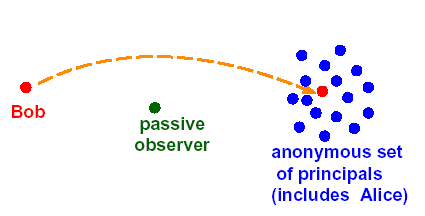
\includegraphics[scale=0.8]{receiver-anon.png}
\end{figure}
If the observer cannot find out whether a given pair of peers
is communicating, Sender-Receiver anonymity is given.
\begin{figure}
    \centering
    \caption[Sender-Receiver Anonymity]{Sender-Receiver Anonymity\\Image source: \protect\url{http://www.cs.virginia.edu/crab/anonymity.ppt}}
    \label{senderreceiveranon}
    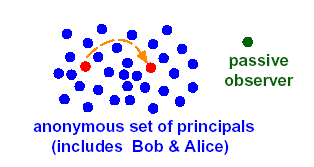
\includegraphics[scale=0.8]{sender-receiver-anon.png}
\end{figure}
The three figures \ref{senderanon}, \ref{receiveranon} and
\ref{senderreceiveranon} visualise the differences.
% -----------------------------------------------------------------------------
\subsection{Sender to receiver anonymity}
Providing anonymity of two people talking to each other is \textbf{not} 
required due to the objectives of this thesis.
% Nico: 1 => reformulate
% -----------------------------------------------------------------------------
\subsection{Receiver identification}
The receiver should be able to verify the identity of the sender, so she
can be sure that the message originated from the correct person.
% Nico: 1 => reformulate
% -----------------------------------------------------------------------------
\section{Confidentiality}
The content of the conversations should be hidden from eavesdropper.
Being able to read the content of messages may also reveal the identity
of the chat partners and thus the anonymity would vanish.
% Nico: 1 => reformulate

% FIXME: solution:
% We encrypt every message via public-key cryptography\cite{pgp-1},
% so that only the receiver can decrypt and view the message content.
% 
% -----------------------------------------------------------------------------
\section{Authenticity}

Know who he/she is and that the message is correct.
As messages may contain important content, it is necessary that the integrity
is guaranteed.
% Nico: 1 => reformulate
% -----------------------------------------------------------------------------
\section{Availability}
Most traditional systems rely on central infrastructure to operate, in which a
single party (like the operator) can disable the service. 
No service can be run reliable, if an attacker with infinite resources is assumed.
Thus the requirement for this chat system is to survive the attack of a single
party and to continue delivering the chat service.
% Nico: 1
% -----------------------------------------------------------------------------
%\section{Non security related features}
%To be able to be compete with other chat protocols, \emph{direct} 
%and \emph{group chat} should be supported.
%\subsection{Direct chat
%implemented by two different chat destinations:
%\begin{enumerate}
%\item \emph{Peers}
%\item \emph{Groups of peers}
%\end{enumerate}
%A peer is just another person (direct chat), a group of peers is the EOF
%equivalent of the IRC channel\cite{irc-1}. As there is no central server,
%groups of peers are managed by each client, and thus the compositions of
%group members may be different on different peers.
%-- 
%Additionally, for practical reasons, EOF must support the following
%chat features:
%\begin{enumerate}
%\item Direct chat ("`message is only seen by one person"')
%\item Group chat ("`message is sent to specific group, which may consist of
%more than one person"')
%\end{enumerate}
% -----------------------------------------------------------------------------
\section{Summary}
\begin{enumerate}
%\item Nobody, but the intended receiver(s) know(s) \emph{that} you wrote a message.
\item Nobody, but the intended receiver(s) can view the \emph{message content}.
\item Nobody, but the intended receiver(s) can \emph{verify} the source of the message being you.
\item Nobody, but the intended receiver(s) know(s) \emph{who} the message was sent to.
\item The network must survive attacks of a single attacker.
%\item Hard (if not practilcally impossible) to block chatting.
\end{enumerate}


